%% This is file `elsarticle-template-1a-num.tex',
%%
%% Copyright 2009 Elsevier Ltd
%%
%% This file is part of the 'Elsarticle Bundle'.
%% ---------------------------------------------
%%
%% It may be distributed under the conditions of the LaTeX Project Public
%% License, either version 1.2 of this license or (at your option) any
%% later version.  The latest version of this license is in
%%    http://www.latex-project.org/lppl.txt
%% and version 1.2 or later is part of all distributions of LaTeX
%% version 1999/12/01 or later.
%%
%% The list of all files belonging to the 'Elsarticle Bundle' is
%% given in the file `manifest.txt'.
%%
%% Template article for Elsevier's document class `elsarticle'
%% with numbered style bibliographic references
%%
%% $Id: elsarticle-template-1a-num.tex 151 2009-10-08 05:18:25Z rishi $
%% $URL: http://lenova.river-valley.com/svn/elsbst/trunk/elsarticle-template-1a-num.tex $



%%
%\documentclass[twocolumn,preprint,authoryear,12pt] {elsarticle}
\documentclass[preprint,authoryear,12pt] {elsarticle}

%\documentclass[preprint,12pt]{elsarticle}
%\smartqed  % flush right qed marks, e.g. at end of proof
\usepackage{graphicx}
\usepackage{subfigure}
\usepackage{amsmath,amssymb,amstext}
\usepackage{soul}
\usepackage{enumerate}
\usepackage{array}
\usepackage{verbatim}
\usepackage{float}
\usepackage{epsf,exscale}
\usepackage[usenames,dvipsnames]{color}
\usepackage{booktabs}
\usepackage{multicol}
\usepackage{tikz}
\usepackage{psfrag}
\usetikzlibrary{shapes,arrows}
\usepackage{mathptmx}      % use Times fonts if available on your TeX system
%\usepackage{amssymb}
%\usepackage{color,graphicx,psfrag,amssymb,amsfonts,amsmath,subfigure,enumerate,float}
\usepackage{ulem}
%\renewcommand{\baselinestretch}{2}
\renewcommand{\baselinestretch}{1}
\usepackage{fullpage}
\renewcommand{\d}{\text{d}}
\renewcommand{\Re}{\text{Re}}
\renewcommand{\Im}{\text{Im}}

\newenvironment{packed_enum}{
\begin{enumerate}
  \setlength{\itemsep}{1pt}
  \setlength{\parskip}{0pt}
  \setlength{\parsep}{0pt}
}{\end{enumerate}}

\newenvironment{packed_item}{
\begin{itemize}
  \setlength{\itemsep}{1pt}
  \setlength{\parskip}{0pt}
  \setlength{\parsep}{0pt}
}{\end{itemize}}

\newenvironment{packed_description}{
\begin{description}
  \setlength{\itemsep}{1pt}
  \setlength{\parskip}{0pt}
  \setlength{\parsep}{0pt}
}{\end{description}}

%===================================
%======= FRONT MATTER =================
%===================================

\journal{UCSC CMPE 216 Bio-Inspired Locomotion (Fall 2018)}

\begin{document}

\begin{frontmatter}

%\title{On the solution of the contact problem involving inhomogeneously elastic bonded layered solids: an analytic approach} 
\title{Hummingbird-Inspired High-Speed Deceleration and Flea-Inspired Vertical Take-Off} 

\author{Pavlo Vlastos \footnote{\textit{pvlastos@ucsc.edu}}}

\address{Baskin School of Engineering, UC Santa Cruz}

%
% REVIEW THIS AFTER WRITING
%
\begin{abstract} 
A design for a bio-inspired robot and simulation are discussed. A flea-inspired jumping mechanism is detailed, in addition to a hummingbird-inspired wing system for accurate navigation and deceleration. The primary goal of the robot is to deliver a fragile payload, an egg, to a desired height and location. This paper reviews similar projects, research, and discusses a novel hybrid approach. The system is split into vertical take-off and controlled gliding.\\
\end{abstract}

\begin{keyword}
Flight \sep Bio-inspired \sep Hummingbirds \sep Fleas
\end{keyword}

\end{frontmatter}

%===================================
%======= PAPER =======================
%===================================

\section{Introduction}
\label{intro}
%===============

Of all the various types of robotic locomotion, a dichotomy can be drawn such that
there are two main categories, robots that require pre-established infrastructure and robots that do not. A rumba requires flat surfaces to traverse, where as DARPA's dog can navigate the uneven surface of a grassy hill. Robots that do not require specific environmental geometry can be deployed in countries that have limited infrastructure to deliver important supplies. For disaster relief, supply delivery via all-terrain, long-distance autonomous vehicles can be critical. \\

This paper outlines a proposal for a high-velocity aerial robot drawing
inspiration from hummingbirds. The robot will use near-vertical take-off, requiring no runway. The bio-inspiration comes from the manner in which humming-birds rapidly decelerate. When hummingbirds are in mating season, the males attract females executing a looping display dive reaching speeds of up to approximately 27 meters per second, \cite{Clark:2009}. The design will incorporate an initial acceleration mechanism to propel the robot to a high altitude. Once the apex of the trajectory is reached, hummingbird-inspired wings and tail feathers will be deployed to mimic the deceleration. \\

The basic design of the robot will be broken up in to two main sections: \textbf{1)} the initial acceleration mechanism and \textbf{2)} the deceleration mechanism. A simulation will first be made, and as a stretch-goal, a prototype will be assembled.

\subsection{Acceleration mechanism}

\section{Formulation of the problem}
\label{Formulation}
%==========================


 	
\section{Method of solution}
\label{method}
%====================

 
\section{Implementation} 
\label{implementation}
%===============

Both the jumping mechanism and wings for deceleration will be outlined here. This section shows possible designs for the robots mechanisms.\\

%===================== Jumping Mechanism ==========
\begin{figure}[H]
\begin{center}
\subfigure[Compressed jumping mechanism]{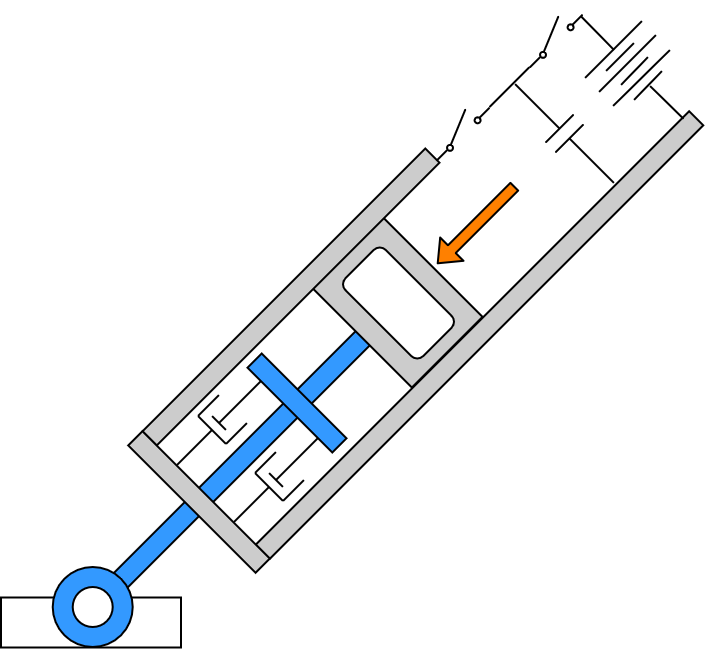
\includegraphics[width=0.4\linewidth]{./Figures/AccelerationMechanism.png} }
\subfigure[Extended jumping mechanism]{\includegraphics[width=0.4\linewidth]{./Figures/AccelerationMechanism2.png} } 
\caption{Example of a chart}
\label{fig:jumpMech}
\end{center}
\end{figure} 
%===================== Jumping Mechanism ==========

\indent The mechanical implementation for the flea-inspired jumping mechanism is shown in \textbf{Figure} \ref{fig:jumpMech}. To achieve the necessary energy density, a small battery and a large capacitor will be used. The capacitor allows for large quantities of charge to be discharged rapidly. The current will flow through the armature, pushing the piston-like leg (blue) out. The micro-controller mentioned in \textbf{section} \ref{method} will control the flow of current and capacitor charging and discharging. \\

%===================== Wings ==========
\begin{figure}[H]
\begin{center}
\subfigure[Folded wings]{
\includegraphics[height=0.3\linewidth]{./Figures/wings2.png} }
\subfigure[Extended wings]{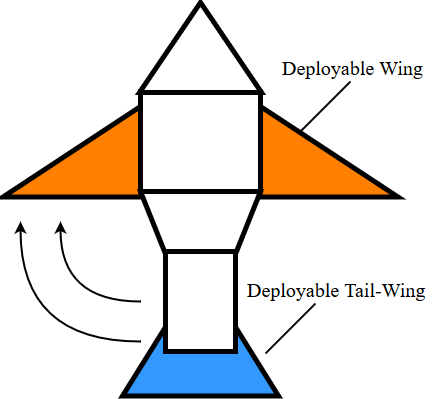
\includegraphics[width=0.4\linewidth]{./Figures/wings.png} } 
\caption{Example of a chart}
\label{fig:wings}
\end{center}
\end{figure} 
%===================== Wings ==========

\indent \textbf{Figure} \ref{fig:jumpMech} shows the deployable wings. The wings must be folded at first to maximize the height. When the wings are folded air resistance is less and the jumping mechanism can propel the robot higher. The on-board micro-controller will control the timing of the wings and when the are deployed.\\ 		
\section{Numerical results and discussions}
\label{results}
%============
\indent When numerical results are prepared, they will be shown here. The acceleration over time, the velocity over time, the position over time, and other information will be graphed and compared to the simulation if the physical robot is constructed.\\
 	

% ADD THIS AT THE END ____
%\section*{Acknowledgement}
% ADD THIS AT THE END ____

% \section*{References}

\bibliographystyle{./model3-num-names.bst}
\bibliography{./TeXFiles/FleaSlug}

\end{document}

